\documentclass[tikz,border=6pt]{standalone}
\usepackage{pgfplots}
\pgfplotsset{compat=1.18}
\begin{document}
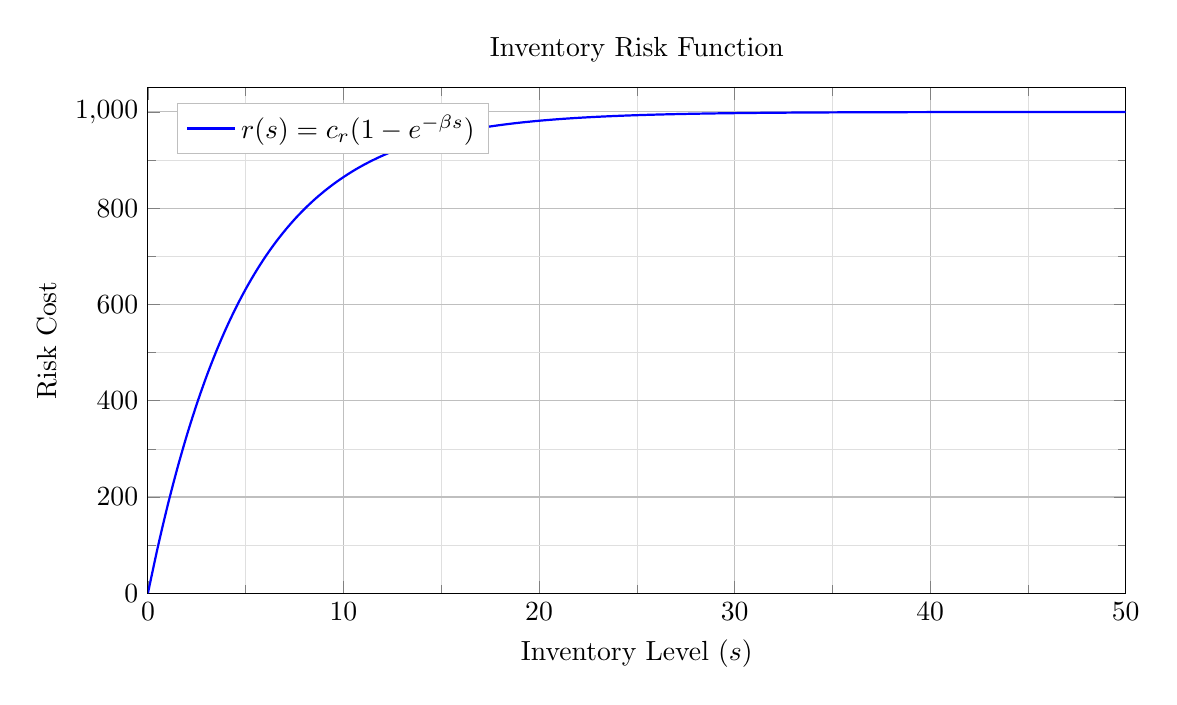
\begin{tikzpicture}
\begin{axis}[
    width=14cm,
    height=8cm,
    title={Inventory Risk Function},
    xlabel={Inventory Level $(s)$},
    ylabel={Risk Cost},
    xmin=0, xmax=50,
    ymin=0, ymax=1050,
    xtick={0,10,20,30,40,50},
    ytick={0,200,400,600,800,1000},
    grid=both,
    major grid style={line width=0.4pt, draw=gray!50},
    minor grid style={line width=0.2pt, draw=gray!25},
    minor tick num=1,
    legend style={
        at={(0.03,0.97)},
        anchor=north west,
        draw=gray!50,
        fill=white,
    },
]
% Parameters: cr=1000, beta=0.2
\addplot[
    smooth,
    thick,
    blue,
    domain=0:50,
    samples=100
] {1000*(1 - exp(-0.2*x))};
\addlegendentry{$r(s)=c_r(1-e^{-\beta s})$}
\end{axis}
\end{tikzpicture}
\end{document}
